\section{Methods}
This section outlines the methods employed to address the problem of domain generalization during training. These techniques were integrated into several model architectures to enhance their performance and provide deeper insights into their behavior under domain shift conditions.
\subsection{MixStyle}
The method introduced by \cite{mixstyle_ref}, known as MixStyle, is a novel, lightweight, and effective module aimed at enhancing the generalization capability of neural networks, particularly in scenarios involving domain shifts and previously unseen data. It addresses a fundamental challenge in machine learning and artificial intelligence - namely, the tendency of models to perform poorly when deployed in environments that differ from the training domain.

\vspace{0.5cm}

\begin{figure}[h]
	\centering
	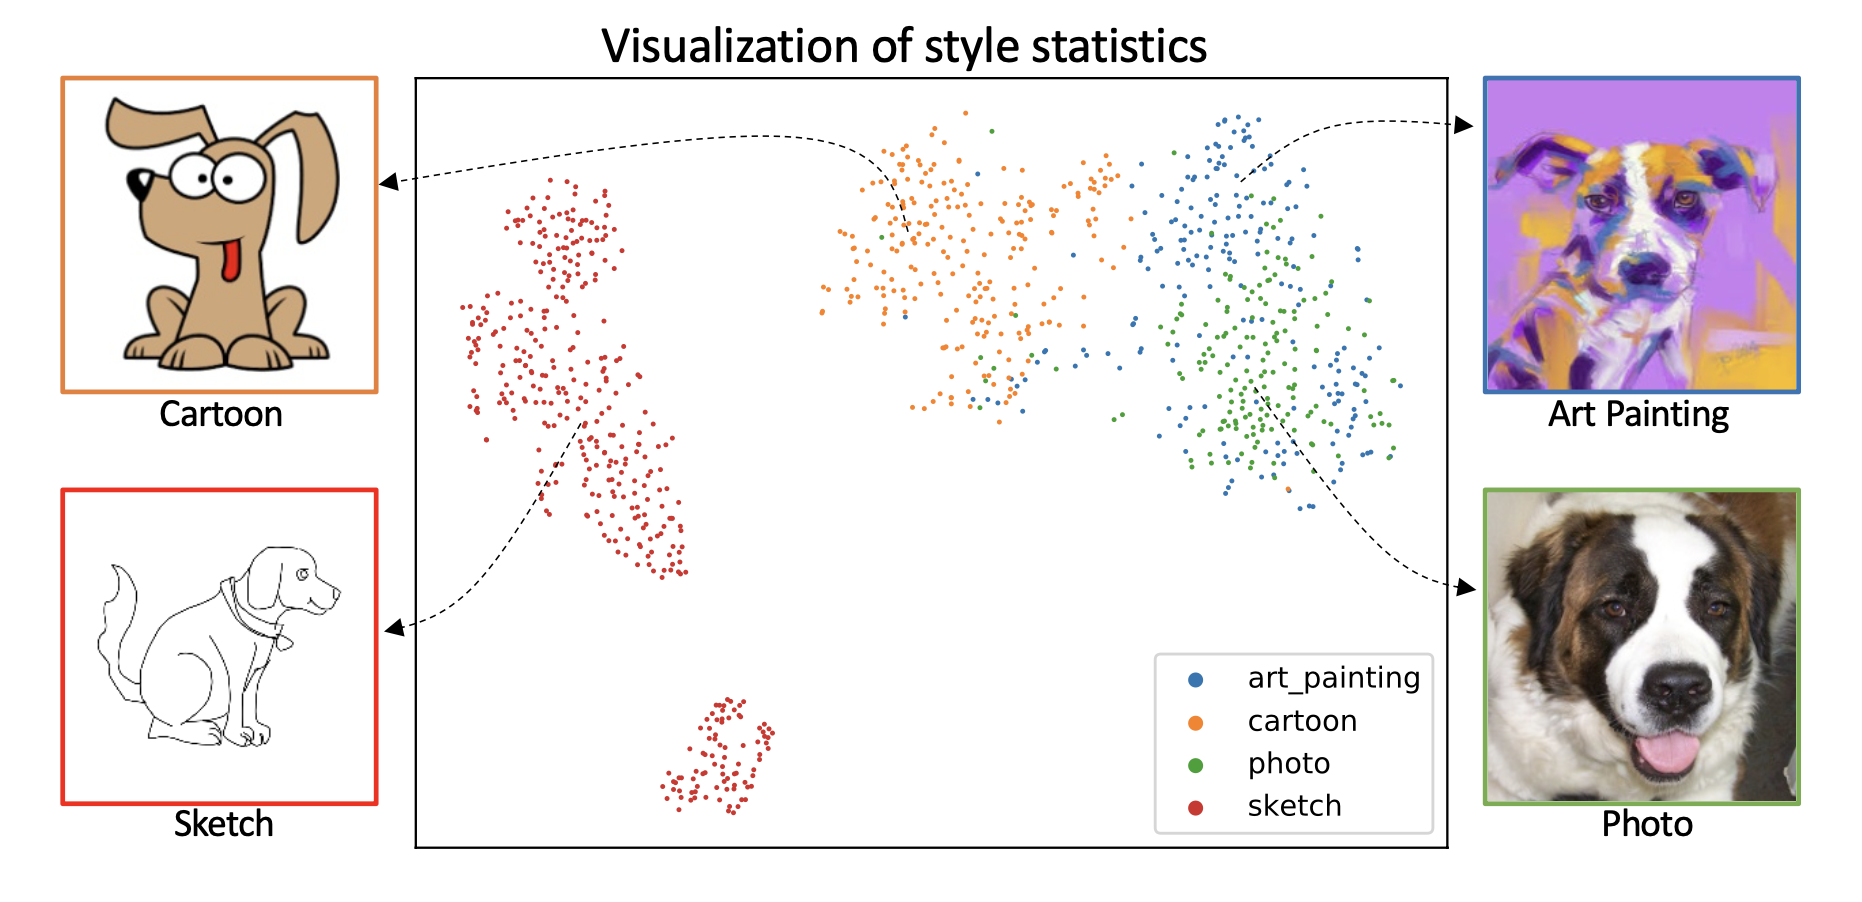
\includegraphics[width=0.5\textwidth]{images/mixstyle_domain.png}
	\caption{Cluster Overview over different domains of the same class.}
	\label{fig:mixstyle}
\end{figure}

\vspace{0.5cm}

The \textit{key idea} behind MixStyle is to simulate domain variability by mixing feature statistics - specifically, the mean and standard deviation - across different samples during training. These statistics extracted in shallow layers of the network capture style-related information, which typically varies across domains. By perturbing them in a structured manner, MixStyle implicitly encourages the network to learn representations that are invariant to style, thereby enhancing its robustness to domain shifts.

As illustrated in Figure~\ref{fig:mixstyle}, style statistics form distinct clusters for different domains. Domain generalization techniques aim to address this by reducing the separation between these clusters. The objective is to align samples of the same class, regardless of their domain origin, into a single, unified cluster. This consolidation of class-specific representations across domains leads to improved generalization and increased classification accuracy on previously unseen domains.

\subsubsection{Image Variablity}\label{susec:variability}
To modulate the degree of mixing between feature statistics from different samples, the authors utilize the $Beta$ distribution to stochastically sample a mixing coefficient denoted by $\lambda$. This coefficient controls the extent to which the style characteristics - specifically, the mean and standard deviation - of each input sample contribute to the resulting mixed representation. A value of $\lambda$ close to 0 or 1 results in an asymmetric combination, where the output is dominated by the style statistics of a single sample, with only a minimal influence from the other. Conversely, when $\lambda$ is near 0.5, the contribution from both samples becomes more balanced, yielding a more homogeneous mixture of their style attributes.

\begin{figure}[h!]
	\centering
	\begin{subfigure}[b]{0.45\textwidth}
		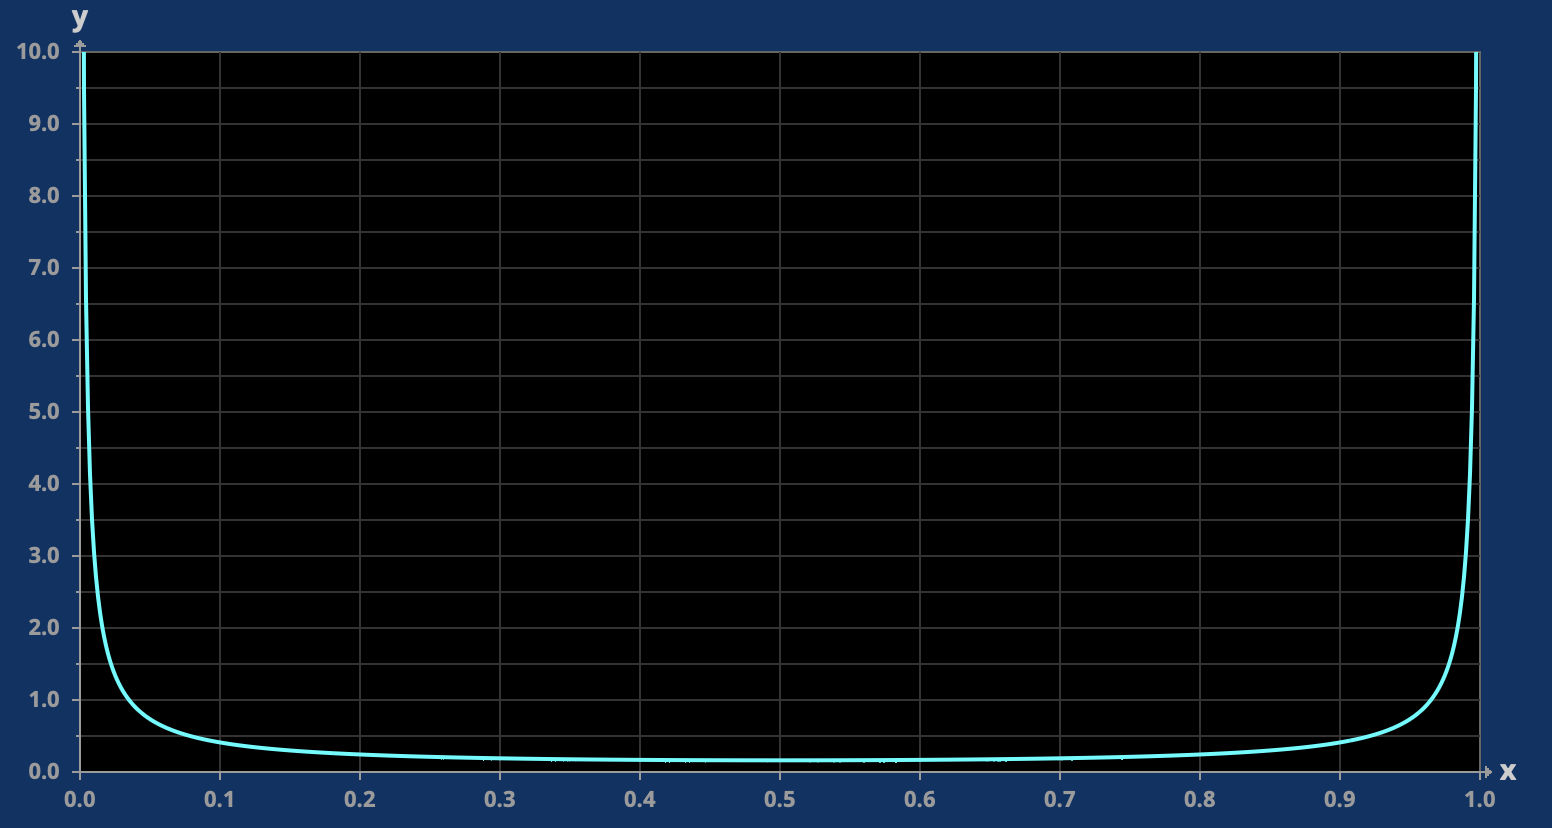
\includegraphics[width=\textwidth]{images/beta01.png}
		\caption{$\alpha = 0.1$}
		\label{fig:alpha01}
	\end{subfigure}
	\hfill
	\begin{subfigure}[b]{0.45\textwidth}
		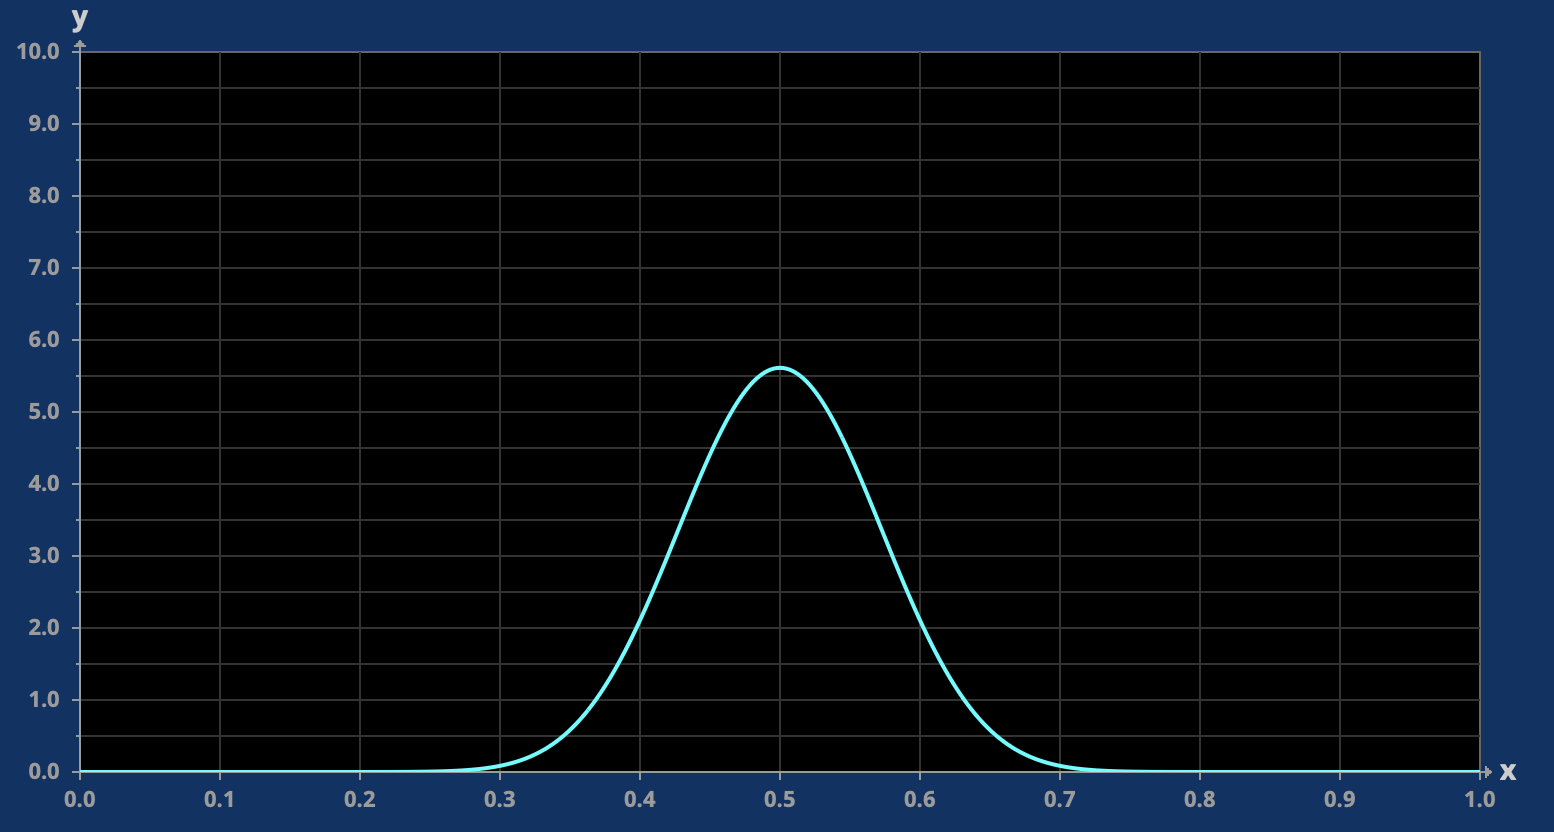
\includegraphics[width=\textwidth]{images/beta25.png}
		\caption{$\alpha = 25$}
		\label{fig:alpha25}
	\end{subfigure}
	\caption{Probability density functions of the $Beta$ distribution with symmetric parameters ($\text{$Beta$}(\alpha, \alpha)$) for different values of $\alpha$.}
	\label{fig:combined_images}
\end{figure}

The value of $\lambda$ is sampled from a symmetric $Beta$ distribution, $\text{$Beta$}(\alpha, \alpha)$, where the hyperparameter $\alpha$ determines the shape of the distribution. For small values of $\alpha$ (e.g., $\alpha = 0.1$) (as shown in Figure \ref{fig:alpha01}), the distribution is U-shaped, assigning higher probability density to values near 0 and 1. This leads to sampled $\lambda$ values that strongly favor one sample over the other, thus resulting in mixed features dominated by the style of a single image. In contrast, larger values of $\alpha$ (e.g., $\alpha = 25$) (Figure \ref{fig:alpha25}) yield a unimodal distribution centered around 0.5, promoting more balanced combinations where the styles of both samples are equally represented. This parameterization allows fine-grained control over the strength and symmetry of feature mixing.

The entire process is applied over mini-batches during training and supports two distinct strategies for selecting image pairs to be mixed. In the random sampling method, pairs of samples are selected at random from the mini-batch, without considering their domain labels. As a result, samples from the same domain may also be combined. In contrast, the cross-domain (xdomain) strategy enforces domain diversity by ensuring that each selected pair consists of samples originating from different domains. This targeted mixing encourages the model to generalize across domain boundaries by explicitly learning representations that are invariant to domain-specific style variations.

\subsubsection{Mechanism}\label{sususec:mechanismmixstyle}

\begin{algorithm}[H]\label{algorithm:mixstyle}
	\caption{MixStyle Operation Forward Pass}
	\KwIn{Feature map $\mathbf{f}$, Feature map $\mathbf{f}'$, parameter $\alpha$}
	\KwOut{Modified feature map $\hat{\mathbf{f}}$}
	Compute mean $\mu$ and std $\sigma$\;
	Sample $\lambda \sim \text{Beta}(\alpha, \alpha)$\;
	Compute mixed $\mu_c$ and $\sigma_c$\;
	Normalize and re-style\;
	\Return{$\hat{\mathbf{f}}$}
\end{algorithm}

The MixStyle layers are positioned immediately after convolutional layers, which are responsible for extracting task-relevant feature representations from the input images.

Given two feature maps, $\mathbf{f}$ and $\mathbf{f'}$, extracted from two different images (potentially from different domains), the first step involves computing the channel-wise mean and standard deviation of each feature map. These statistics are calculated over the spatial dimensions of each channel as follows:

\begin{equation}
	\mu_c = \frac{1}{HW} \sum_{h=1}^{H} \sum_{w=1}^{W} x_{c,h,w}, \qquad
	\sigma_c = \sqrt{ \frac{1}{HW} \sum_{h=1}^{H} \sum_{w=1}^{W} (x_{c,h,w} - \mu_c)^2 }
\end{equation}

Here, $x_{c,h,w}$ denotes the activation at channel $c$ and spatial location $(h, w)$, while $H$ and $W$ represent the height and width of the feature map, respectively. The computed $\mu_c$ and $\sigma_c$ describe the style characteristics of the input sample, inspired by style transfer techniques where such statistics are associated with visual appearance.

Following the computation of these style statistics, a mixing coefficient $\lambda$ is sampled from a Beta distribution, as described in Section \ref{susec:variability}. This coefficient determines the extent to which the style from one sample is combined with that of another. Specifically, $\lambda$ determines whether the resulting feature representation is a strong interpolation of both styles (when $\lambda \approx 0.5$), or largely dominated by one (when $\lambda$ is close to 0 or 1). 

\begin{equation}\label{formula:2}
	\gamma_{\text{mix}} = \lambda \, \sigma(\mathbf{f}) + (1 - \lambda) \, \sigma(\mathbf{f}') \\ ;
	\beta_{\text{mix}} = \lambda \, \mu(\mathbf{f}) + (1 - \lambda) \, \mu(\mathbf{f}') \\
\end{equation}

Equation~(\ref{formula:2}) define the computation of the mixed feature statistics used in the MixStyle transformation. Specifically, the mixed standard deviation $\gamma_{\text{mix}}$ and mixed mean $\beta_{\text{mix}}$ are obtained through a random convex combination of the channel-wise statistics from the two feature maps. 

\begin{equation}\label{formula:3}
	\hat{\mathbf{f}} = \gamma_{\text{mix}} \odot \frac{\mathbf{f} - \mu(\mathbf{f})}{\sigma(\mathbf{f})} + \beta_{\text{mix}}
\end{equation}

The final output feature map of each MixStyle layer is computed as shown in Equation~(\ref{formula:3}), where the original feature representation $\mathbf{f}$ is combined with the feature statistics - mean and standard deviation - extracted from a second, randomly selected sample. This mixing process introduces stochastic style variations during training while preserving the semantic content of the features.

The purpose of this stochasticity is to simulate domain shifts in a controlled manner, thereby forcing the model to learn representations that are invariant to domain-specific style variations. By disentangling style from content, MixStyle helps the network generalize more effectively to previously unseen domains.

\subsubsection{Benefits}
The MixStyle method demonstrates several key advantages described by \cite{mixstyle_ref} supported by extensive experimental results. First, it significantly improves domain generalization, consistently outperforming vanilla ResNet-18 and other regularization techniques on benchmark datasets. Specifically, MixStyle achieves approximately a 4\% increase in accuracy on the PACS dataset and a 1\% improvement on Office-Home compared to the traditional Mixup method. This performance gain is notable given the method’s simplicity, which also allows it to surpass more complex approaches such as L2A-OT by nearly 1\% on PACS.

MixStyle exhibits particular strength in low-data regimes, delivering over 6\% improvement with only 10 labels per class and nearly 7\% improvement with 5 labels per class on PACS, demonstrating its effectiveness in scenarios with limited training data. Additionally, the method’s versatility is evident as it achieves strong results not only in supervised learning environments but also in unsupervised and semi-supervised domain adaptation settings.

However, while MixStyle excels on smaller datasets, it does not outperform more advanced methods like L2A-OT on larger datasets such as Office-Home when applied alone, indicating opportunities for further refinement or combination with complementary techniques.

\subsubsection{Integration}
Based on the assumption that domain-related style statistics are more prominent in the shallow layers of convolutional neural networks (CNNs), MixStyle should be integrated into earlier layers of the architecture. For instance, in ResNet architectures, the optimal configuration involves inserting MixStyle behind the first and the second residual blocks. This setup enables the synthesis of "new domains" without disrupting the semantic representations required for the primary task - such as image classification - which are typically learned in deeper layers.

\cite{mixstyle_ref} recommend this configuration across different task settings. Specifically, for object recognition, they found that placing MixStyle after residual Blocks 1, 2, and 3 yields the best performance. Our setup, as detailed in Section~\ref{sec:setup}, follows a similar approach for image classification tasks. In contrast, introducing MixStyle in later layers leads to a decline in performance, likely due to the mixing of high-level semantic features, which negatively affects classification accuracy.

The implementation, as described in Section~\ref{sususec:mechanismmixstyle}, is structured around a Python module that defines the mathematical operations of MixStyle within the forward function as shown in Listing~\ref{listingMixstyle}. This design ensures that all computations are executed during the forward pass. Additionally, a new module was introduced to encapsulate the various model architectures used during training and evaluation. Within this module, a parent class was defined for each model, extended with parameters that specify the insertion points of the MixStyle layers. This modular and parameterized approach enables seamless integration of MixStyle into different architectures, making it well-suited for use during model training.

\begin{lstlisting}[language=Python, caption={MixStyle implementation structure}, label=listingMixstyle]
class MixStyle(nn.Module):
	...
	def __init__(self, p=0.5, alpha=0.1, eps=1e-6, mix="random", seed=42):
	...
	
	def forward(x):
	...
\end{lstlisting}

To support the integration of MixStyle into various model architectures, an additional module was developed to encapsulate and manage different network configurations used for training and evaluation. This module defines a parent class for each model, extended with parameters that allow precise control over the insertion points of MixStyle layers. These configurations are predefined and stored under specific model names that also encode additional details such as the position of MixStyle layers and the setup of the final classification layer.

As illustrated in Listing~\ref{listingModelLoading}, model instances can be easily loaded by referencing their respective names from the \texttt{resnet\_ms} module. This approach ensures a flexible and reproducible training pipeline, as each model variant is preconfigured with consistent parameters.

\begin{lstlisting}[language=Python, caption={Model loading from predefined configurations}, label=listingModelLoading]
	MODEL = resnet_ms.resnet50_fc512_ms12_a0d1
\end{lstlisting}

To facilitate experimental reproducibility and ease of use, the most effective architectures were encapsulated as callable model definitions. These predefined models can be conveniently loaded within Jupyter notebooks or scripts, enabling seamless execution of various training and evaluation scenarios across different configurations. 
